% ================
% Landon Buell, Kevin Short
% JMM Paper
% PHYS 705.01 - Lab00
% 21 Sept 2020
% ================

\documentclass[conference,twocolumn,letterpaper]{IEEEtran}

\usepackage{amsmath,amssymb}
\usepackage{graphicx}
\usepackage{cite}
\usepackage{color}
\usepackage{subfigure}
\usepackage[top=1.5cm,left=1.5cm,right=1.5cm]{geometry}

% ================================================================

\title{Musical Instrument Classification Using a Hybrid Neural Network}
\author{Landon H. Buell$^1$ and Kevin M. Short$^2$ \\
        $^1$lhb1007@wildcats.unh.edu and $^2$kevin.short@unh.edu\\
        $^1$Department of Physics and Astronomy\\
        $^2$Department of Mathematics and Statistics\\
        University of New Hampshire, Durham, New Hampshire, USA \\}
\date{December 2020}

% ================================================================

\begin{document}

\maketitle

% ================================================================================================================================

\begin{abstract}
    Classifying audio signals with machine learning has become an important topic of research in the past few years. Models often involve the input of a 2-D spectrogram or 1-D feature vector into a unimodal network such as a Convolutional Neural Network (CNN) or Multilayer Perceptron (MLP). In this study, we explore automatic classification of musical instruments using new hybrid neural-network architecture that combines the CNN and MLP models and provides superior performance over models that rely solely on one or the other. This hybrid network uses two branches, one being a CNN to process an image-like 2-D spectrogram, and the other being an MLP to process a 1-D feature vector. Within the model, a hidden layer combines activations from the two branches by concatenating them into a single 1-D dense layer, thus all predictions are a product of both branches. We describe in detail the creating of the spectrogram and features, as well as how they influence the chosen network architecture. We finish with a practical demonstration that uses this classifier model to match waveforms from a chaotic music synthesizer to real-world musical instruments. Training data is from studio recordings of the Philharmonia Symphony Orchestra and University of Iowa's Electronic Music Studios
\end{abstract}

% ================================================================================================================================

\section{Introduction}
\label{sec:Intro}

% ================================================================

Digital audio analysis and classification has become a very prolific field in the last few years. The exact nature of each task can differ drastically from archival management, to security, or to commercial usage. In each case, we seek to place audio files into distinct categories called \textit{classes} based in inherent properties within the data \cite{James,Khan,Liu}. Consider a collection of audio files, each containing a single note performed by some musical instrument and the task of matching the contents of the file to the instrument that it most closely resembles. This type of classification task is near trivial for humans, but given the volume of audio data in the modern world, it is impractical at a large scale. However, a computer has no difficulty processing large volumes of raw information, but encoding an explicit instruction set for classification is unreasonable. For this reason, we turn to a \textit{neural network} to combine the computational efficiency of a computer, with the decision-marking architecture of a brain \cite{Geron}. 

A neural network is a machine learning model that allows a set of inputs, $x$, called \textit{features}, to be transformed into a set of outputs, $y$,  called \textit{predictions} using a set of \textit{parameters}, $\Theta$ \cite{Geron,Goodfellow,Virtanen}. Audio classification with machine learning is also a well-explored field, with much research in developing an appropriate set of features, also called \textit{predictors}, for input \cite{James,Liu,Mierswa,Zhang}. Since the each classification task or data set may differ greatly from any other, each model often requires a unique combination of features which allows for the best possible performance \cite{Virtanen}. For musical instrument classification we have chosen predictors that represent the contents of an audio file using two different \textit{modalities}. We call this type of classification \textit{multimodal learning} \cite{Ngiam}.

Multimodal learning differs from other types of supervised learning in that a model accepts and processes multiple inputs that are each different representations of the same data sample. Data sets that include or can be transformed into audio + visual, audio + text, or even text + text information, are all examples of multimodal data sets \cite{Li}. For digital audio classification, we have chosen to represent the contents of an audio file by decomposing it into \textit{image + vector} information format. We do this by constructing a 2D spectrogram and a 1D vector of features from the same waveform. Data from these different modes encodes complementary information which allows a model to develop parameters that can more thoroughly describe a sample when compared to it's unimodal learning methods \cite{Li}

To account for this multimodal input, we have constructed a \textit{hybrid neural network} that utilizes two input branches, each with its own set of layers to process an input mode. The spectrogram image is transformed with a Convolutional Neural Network (CNN) which uses layers of 2D convolution and 2D pooling to generate a feature map, which is then flattened and transformed by repeated matrix-vector equations, this is visualized on the left side of Fig. (\ref{fig:Architecture}). The feature vector input is transformed through multiple matrix-vector equations which can be seen on the right side of Fig. (\ref{fig:Architecture}). The activations for each sample in each branch are concatenated into a single layer, which is further transformed into a single output prediction found at the bottom on Fig. (\ref{fig:Architecture}). This means that the neural network learns a set of parameters which allows for mapping of \textit{both} input modes into a single prediction. Since the properties of the input features are critically important to classification success, multi-representation learning shows a great deal of promise and wide spread applicability \cite{Khan,Li,Liu,Virtanen}. We find the the implementation of this hybrid architecture demonstrates an average superior classification performance when compared to either of its constituent unimodal architectures.

% ================================================================================================================================

\section{The Neural Network}
\label{sec:NeuralNetwork}

% ================================================================

\subsection{Structure}
\label{subsec:Intro}

A neural network is a type of machine learning algorithm that is inspired from the human brain \cite{Geron,Goodfellow}. Where biological brains are constructed from neurons and connected through axons, neural networks are constructed from artificial neurons and connected through weighting functions. 




% ================================================================

\subsection{Input and Output}
\label{subsec:InputOutput}

The inputs to a neural network or any machine learning algorithm are called \textit{features} or \textit{predictors} \cite{James}. These are compact, low-dimensional representations of a data sample reflect its important characteristics \cite{Liu}. Features should be chosen as to have low variance within each class and high variance between classes. For digital audio classification of musical instruments, features of the same musical instruments should exhibit very similar properties, while features from difference musical instruments should exhibit non-similar properties. In any learning algorithm, the role of feature extraction is to translate the raw information into descriptors that maximize the classification performance \cite{Virtanen}. Although the neural network will classify the musical instrument within the digital audio sample, it will never interact with the raw waveform directly, instead will rely solely on these features. Suppose we use $p$ predictors, for a classifier model. These features are usually combined into a single vector-like object for each sample, and then presented as input to the neural network \cite{Geron}. We detail the classification features for this neural network in section (\ref{subsec:Features}). 

The outputs to a classification neural network encodes the prediction that model has made for a particular sample. For a classifier with $k$ classes, there are $k$ output neurons transformed such that the sum of the activations 
neurons to be treated as a probability density \cite{Goodfellow,James}.  The neuron with the highest activation value is the class that it is chosen to belong to. For classification of musical instruments, each class represents a musical instrument type. We use $37$ classes of instruments ranging from woodwinds, to brass, to strings, to mallet percussion, to synthesizers. Each audio file contains exactly one musical instrument sustaining one note.

% ================================================================

\subsection{The Cost Function}
\label{subsec:CostFunction}

A neural network is trained by providing a batch of input samples $X$, with a corresponding set of expected predictions $Y$. Each sample $x$ in the batch input is expected to produce the label $y$, and when passed through the network, creates the prediction $y^*$. For an untrained network, we anticipate that $y^*$ and $y$ may differ greatly- meaning that the prediction is very different that the expected output, and classification performance is likely to be very poor. Since we know each sample in the data set to contain one, and only one musical instrument, we \textit{one-hot-encode} the expected label $y$. For any sample $x^{(i)}$ that belongs to class $j$, we have a corresponding target vector $y^{(i)}$ given by:
\begin{equation}
    \label{eqn:OneHotEnc}
    y^{(i)} = \big[ y_{0} , y_{1}, ... , y_{j}, ... , y_{k-1} \big] = \big[ 0, 0, ... , 1, ... , 0 \big]
\end{equation}
The same sample will produce a similarly sized vector, $y^{*(i)}$, which all elements sum to $1$.

To quantity the difference between $y$ and $y^*$, we introduce a \textit{cost function}, $J(y,y^*)$ which is also called an objective function or a loss function \cite{James}. The exact cost function used can differ based on the nature of the machine learning model or task, but typically multiple - category classification tasks use a \textit{categorical cross-entropy} (CXE) function \cite{Geron,Goodfellow}. The CXE cost for a single sample is defined as \cite{Goodfellow,Virtanen}:
\begin{equation}
    \label{eqn:CXELoss}
    \text{CXE}[y,y^*] = - \sum_{i=0}^{k-1} y_{i} \ln(y^*_{i})
\end{equation}
Since $y$ is one-hot-encoded, the only non-zero term in the sum is $y_{j} \ln(y^*_{j})$, where $y^*_{j} \in [0,1]$ This returns a negative number, which we multiple by $-1$ to always yield a positive cost. When a sample produces $y^*_{j} << 1$, the CXE cost returns a large value and when $y^*_{j} \approx 1$, then the CXE cost returns a small value. We provide a visualization of this behavior in Fig. (\ref{fig:CXELoss}).

\begin{figure}[h]
    \centering
    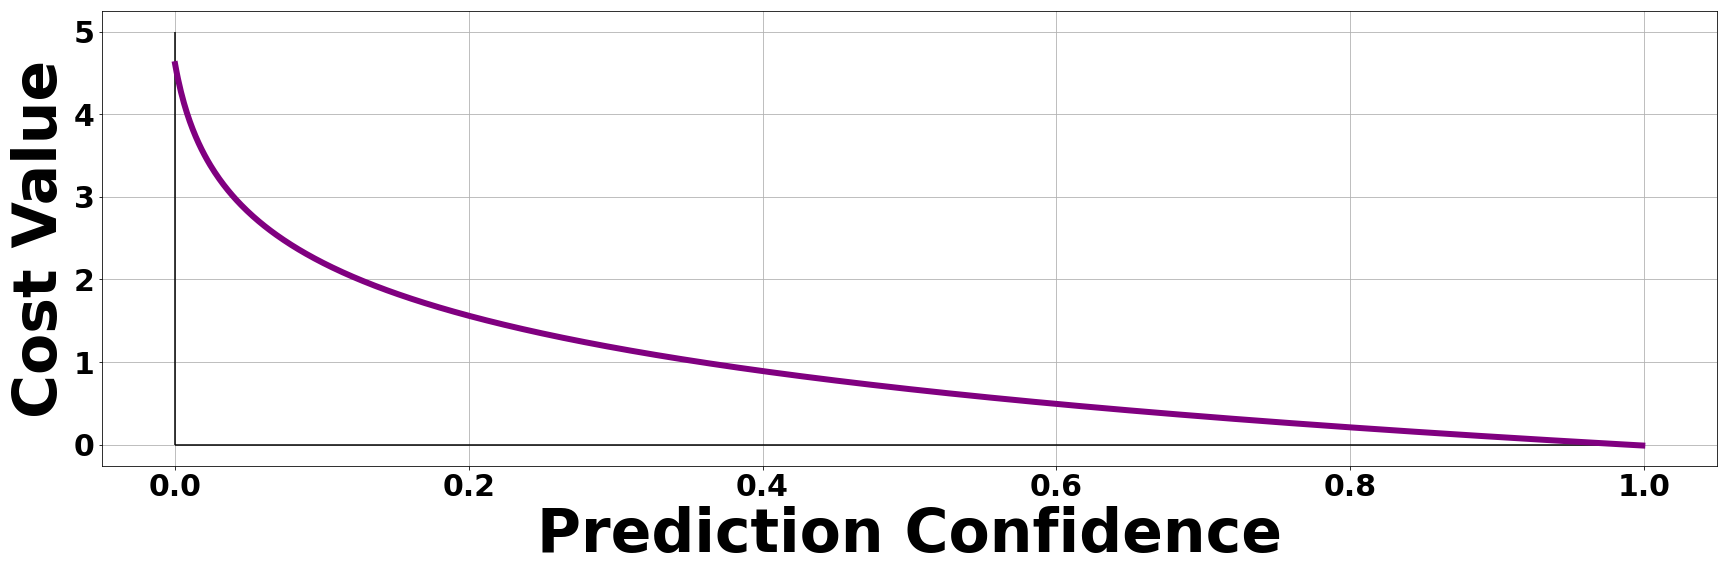
\includegraphics[scale=0.14]{figures/CXELoss.png}
    \caption{Categorical Cross Entropy Cost Function given values for $y^*_{j} \in [0,1]$}
    \label{fig:CXELoss}
\end{figure}

We characterize the cost function as producing a value inversely proportional to the prediction confidence- A large cost value indicates a \textit{poor} prediction label and a low cost value indicates a \textit{good} prediction label \cite{James,Virtanen}. Thus, we expect a trained neural network to produce consistently low cost function values across all samples in a data set. When a neural network does return consistently low cost function values for previously unseen samples, we consider it to be a \textit{fitted} or \textit{trained} network \cite{Geron,Goodfellow,James}.

% ================================================================

\subsection{The Training}
\label{subsec:CostFunction}

A neural network makes predictions by successive transformations of input features through layer functions until a final output array is produced. Each layer $f^(l)$, of the model is a function that contains a set of parameters $\Theta^{(l)}$ which is used to transform activations which are passed to the next layer in the chain \cite{Goodfellow}. The process of training the network is the manipulation of these parameters in each layer, such that each input $x$ can produce a reasonably accurate output, $y^*$. Since we can quantify the difference between the expected output and the given output with a cost function, we can use this as a metric for measuring how "trained" a model is \cite{James}. Specifically, we train a neural network by \textit{optimizing} the parameters in each layer to allow for this consistently low cost function value \cite{Geron}. Note that although we are interested in classification performance, we instead optimize the cost function under the assumption that doing so will also improve the performance. This is called indirect optimization \cite{Goodfellow}.

Since a the function chain that comprises a neural network can become exceedingly complicated for deeper and wider networks, producing a single analytical expression for the optimization of every single is either impractical or impossible. We instead optimize the network with a numerical iterative-based method called \textit{gradient descent} \cite{Geron,Goodfellow}. Gradient descent is the process of (i.) computing the gradient of the cost function with respect to every element in $\Theta$ and (ii.) adjusting each parameter in $\Theta$ according to the gradient. This is typically done with groups of samples at the same time called \textit{batches} to improve computational efficiency. 

% ================================================================================================================================

\section{Features and the Multimodal Network}
\label{sec:Features}

% ================================================================

\subsection{Convolutional Network Features}
\label{subsec:Features}

A spectrogram is a 2D representation of the energy distribution as a function of time and frequency in a periodic waveform-like signal \cite{Virtanen}. The spectrogram is particularly useful because it allows us to examine the frequency composition of a signal, and how that composition evolves over time. On a typical spectrogram, the passing on time is shown on the x-axis, and frequency is shown on the y-axis. Because it is represented as a 2D array or floating-point numbers, the spectrogram is effectively an image-like representation of a sound wave. Since each musical instrument produces it's own harmonic structure, and transient response, each instrument can be identified by patterns within the spectrogram. This means than when only use this modality, the audio classification becomes very similar to an image classification task \cite{Ngiam}. We provide a few example spectrograms for reference in Fig. (\ref{fig:Example Spectrograms}).

\begin{figure}[h]
    \centering
    \subfigure[]{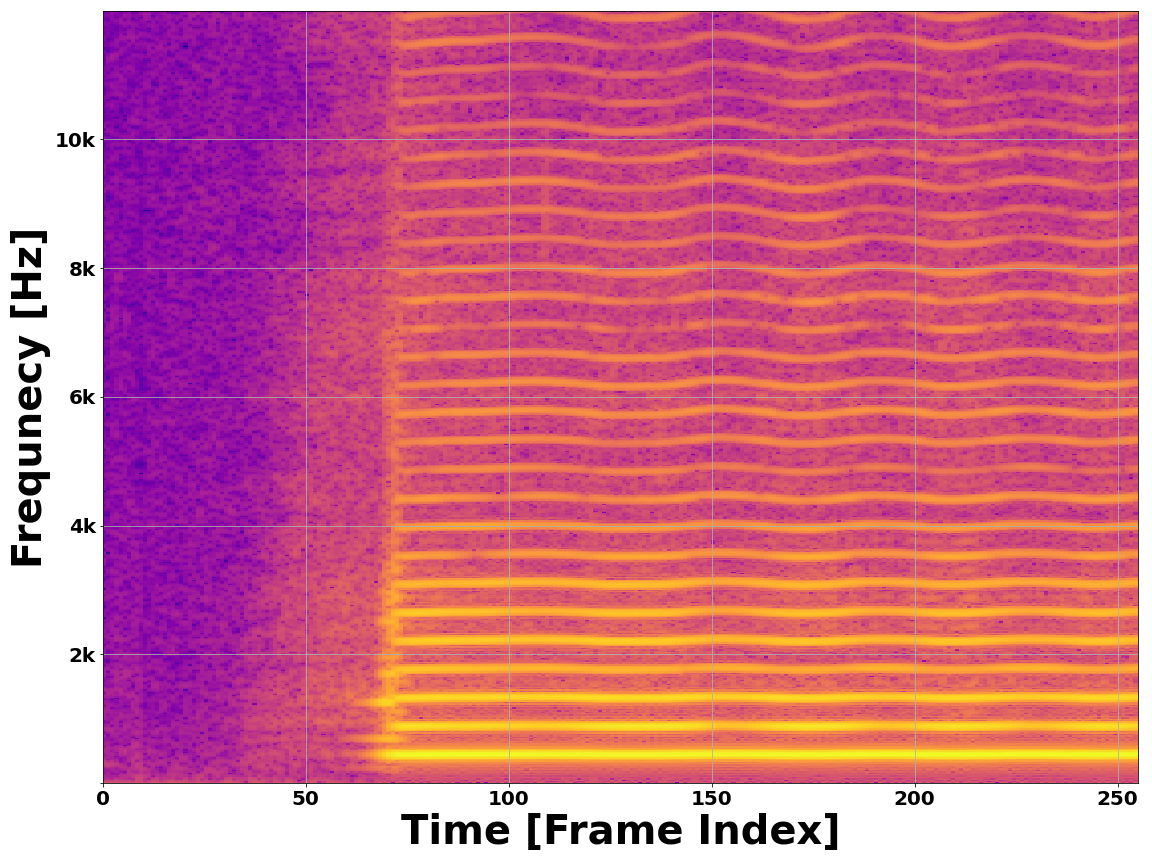
\includegraphics[width=0.45\textwidth]{figuresSpectrograms/AltoSax-A4.png}}
    \subfigure[]{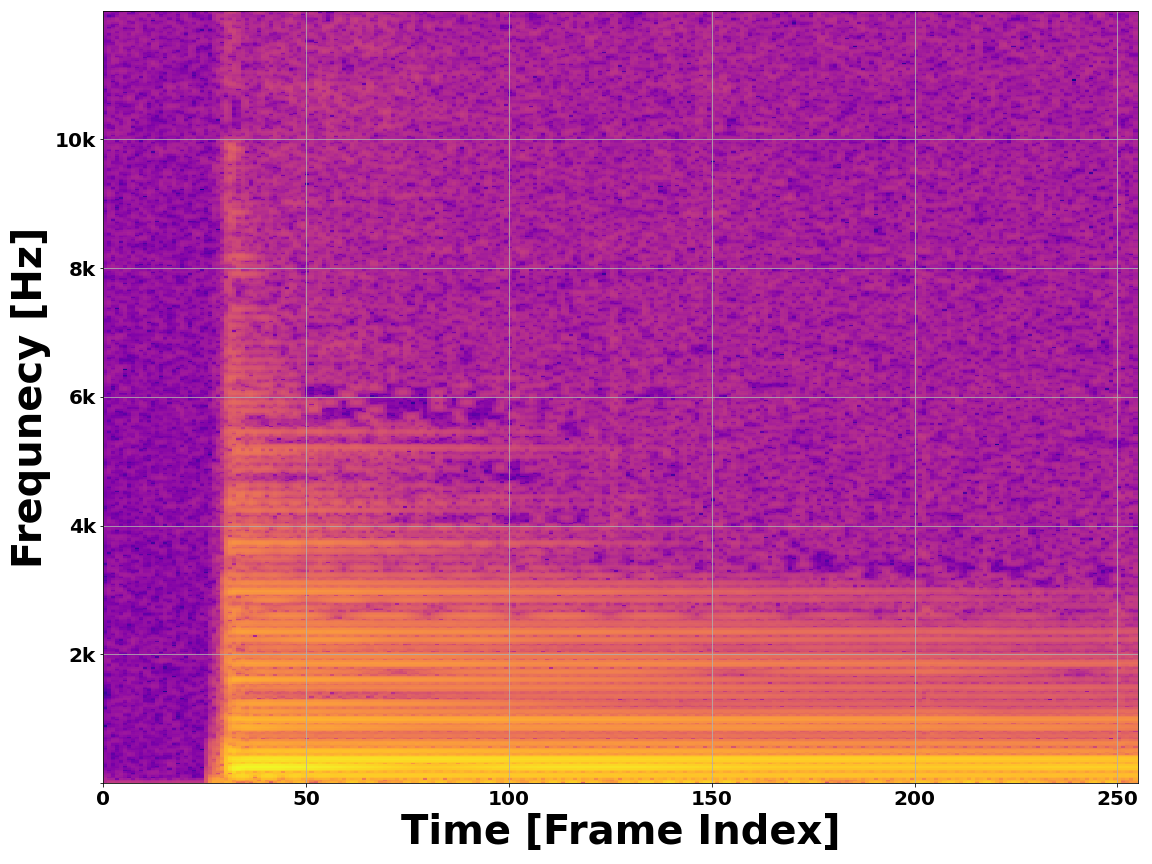
\includegraphics[width=0.45\textwidth]{figuresSpectrograms/GUITAR-B2.png}}
    \caption{Spectrograms of (a) an alto saxophone playing an $A4$ and (b) an acoustic guitar playing a $B2$}
    \label{fig:Example Spectrograms}
\end{figure}

A spectrogram is produced by applying the technique of \textit{frame-blocking} to a waveform to produce a matrix of short-time analysis frames \cite{Liu,Virtanen}. We choose each frame to contain $N = 1024$ samples, with a $768$ sample overlap between adjacent frames. 
\begin{figure}[h]
    \centering
    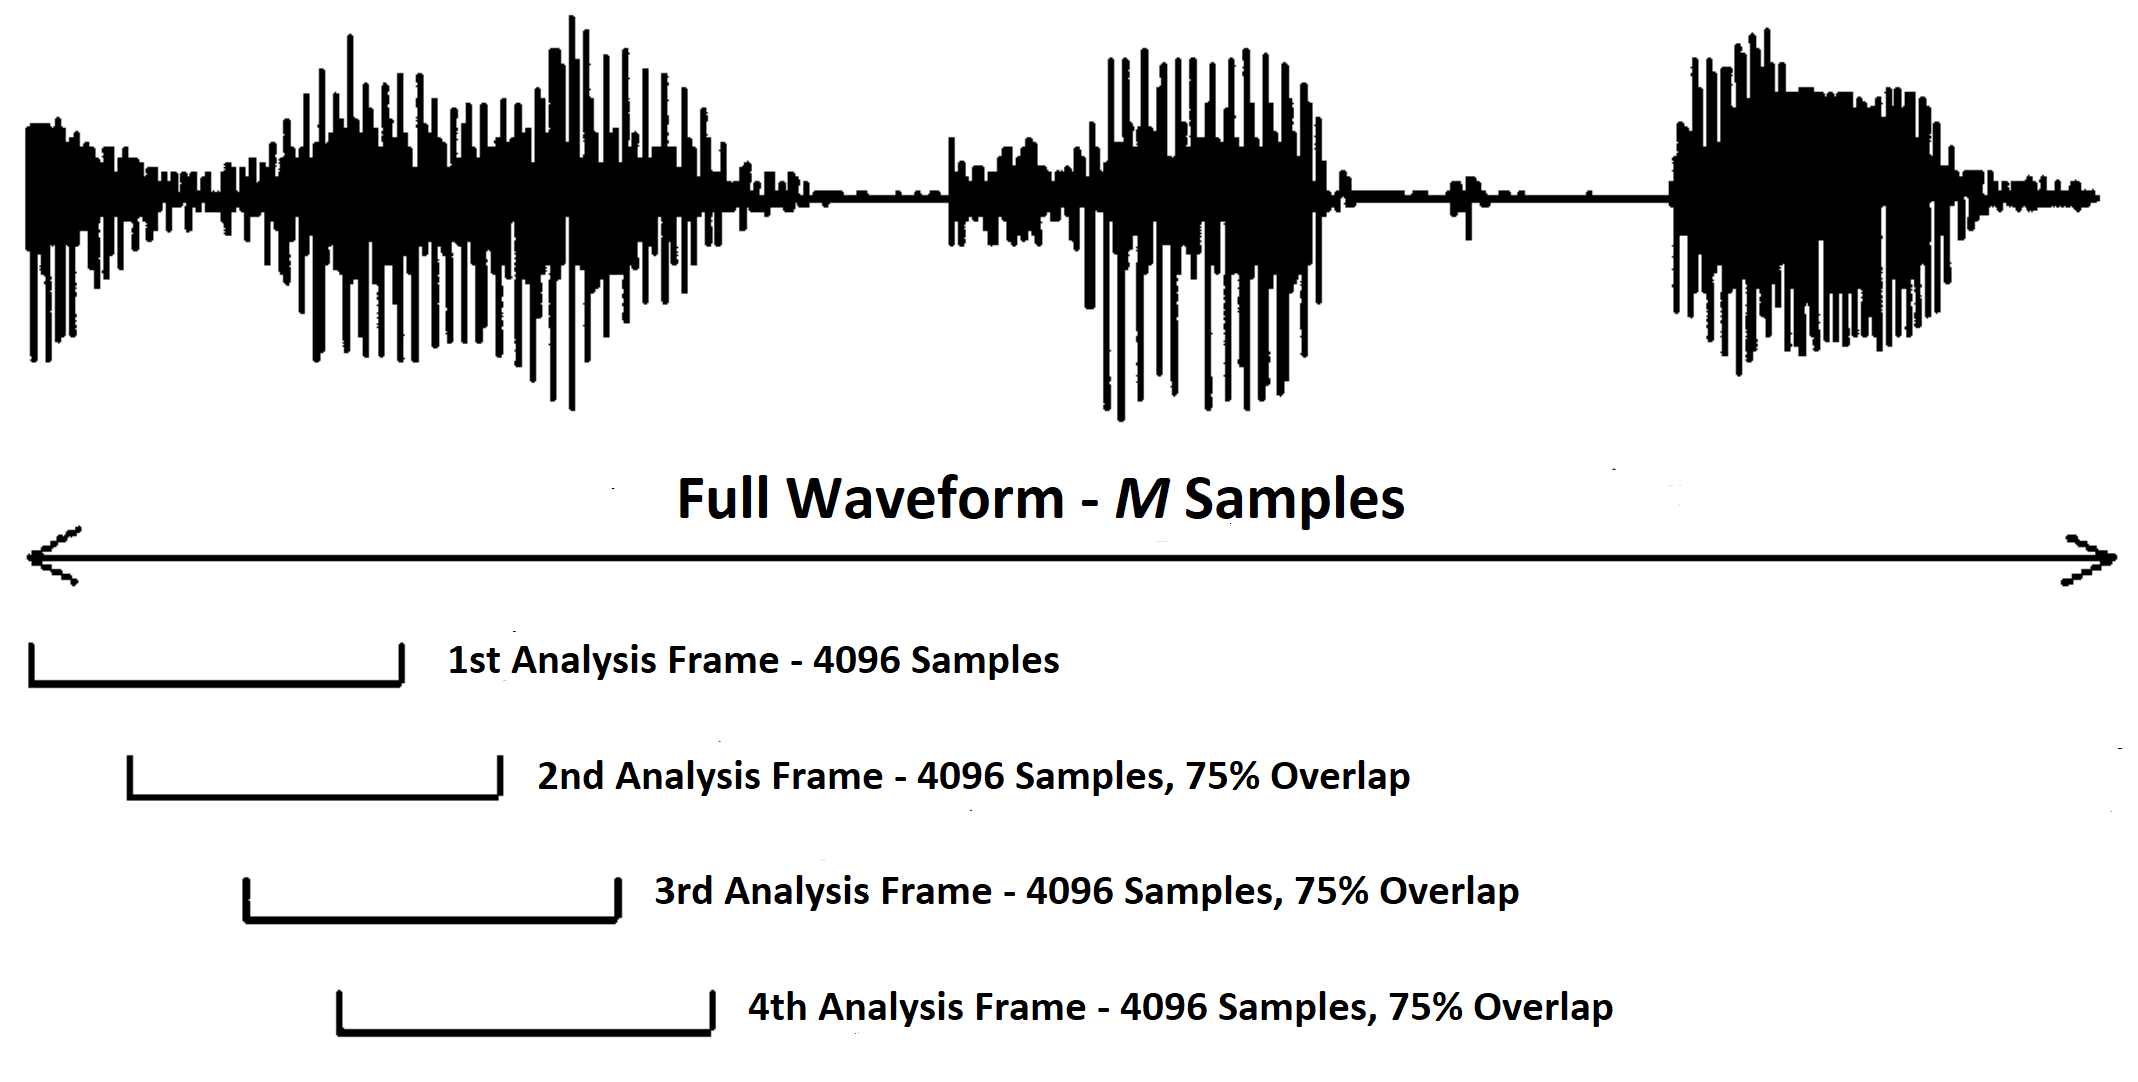
\includegraphics[width=0.45\textwidth]{figures/AnalysisFrames.png}
    \caption{Analysis frames in relation to a full waveform. This figures has been adapted from \cite{Liu}.}
    \label{fig:AnalysisFrames}
\end{figure}
We organize the analysis frames into a matrix, $A$ with shape $N \times k$, such that each row is a frame. We apply a Hanning window of length $N$ to each row of $A$. This eliminates discontinuities at the edges of each analysis frame, and allows for a cleaner transform into frequency-space \cite{Virtanen}. 



% ================================================================

\subsection{Multilayer Perceptron Features}
\label{subsec:Features}

The feature is this section are derived from the time-domain or frequency-domain representation of a waveform. Each feature explored represents the values computed from each audio file, which are then assembled into a 1D array-like object called a feature vector. This vector is provided as input to the MLP branch of the neural network, which can be found on right side of Fig. (\ref{fig:Architecture}). To ensure a consistency of all extracted features, all waveforms have been truncated or zero-padded to contain a consistent $M$ samples.

\begin{enumerate}

\item\textbf{Time Domain Envelope} (TDE) - 
The TDE is a method of approximating the energy in the full or subset of the time-series waveform of a signal. We divide the waveform into $5$ non-overlapping analysis frames and compute the RMS energy of the waveform in each section. This allows for an approximation of the amplitude envelope of the time-domain signal \cite{Virtanen}. For a signal $s$, the RMS energy in the $j$-th frame containing $Q$ sample sis given by:
\begin{equation}
    \label{eqn:TDE}
    \text{TDE}_j[s] = \sqrt{\frac{1}{Q}\sum_{i=n}^{n+Q}s[i]^2}
\end{equation}
These features allow us to characterize the time-evolution of energy in a signal. Instruments with heavy attacks, and sudden decays show large TDE values in early frames, and low TDE values in later frames. Instruments with longer sustains will show consistently decaying TDE values throughout the duration of the file.

\item\textbf{Zero Crossing Rate} (ZXR) - 
The ZXR of a waveform measures how many time that a signal crosses it's equilibrium value, often normalized per unit time. This feature is commonly used to differentiate speech from music because speech often has a more jagged and less periodic structure, giving it a characteristically higher ZXR value \cite{Virtanen,Khan,Zhang}. We adapt this feature to compute the zero-crossing rate over the full waveform. The zero crossing rate for a waveform $s$ with $M$ samples is given by:
\begin{equation}
    \label{eqn:ZXR}
    \text{ZXR}[s] = \frac{1}{2}\sum_{i=i}^{M-1}\Big| \text{sign}\big(s[i]\big) - \text{sign}\big(s[i-1]\big) \Big|
\end{equation}
Where $\text{sign}(x)$  returns $+1$ if $x > 0$, $−1$ if $x < 0$ and $0$ if $x = 0$. In generally, the zero crossing rate can also be used as a rough frequency measurement, where instruments that can produce higher fundamental frequencies often have higher ZXR values, where instruments that can produce lower fundamental frequencies have lower ZXR values \cite{Zhang}.

\item\textbf{Temporal Center of Mass} (TCM) - 
The TCM of a waveform computes approximately where in time, the energy of a waveform is centered around, and can conveniently summarize characteristics of the transient response into a single scalar value. The temporal center of mass of a signal $s$ with $M$ samples is given by:
\begin{equation}
    \label{eqn:TCM}
    \text{TCM}[s] = \frac{\sum_{i=0}^{M-1}i\big|s[i]\big|}{\sum_{i=0}^{M-1}\big|s[i]\big|}
\end{equation}
For instruments with heavier attacks and short decay and release times, such as plucked strings or percussion, we expect the energy of the waveform to be very early on, thus providing a very low TCM value. For instruments with shorter attacks, with long sustain and release times, such as bowed strings or woodwinds, we expect the energy of the waveform to be more spread out, thus have a higher TCM value.

\item\textbf{Auto Correlation Coefficients} (ACC) -
ACC's are rough estimates of the signal spectral distribution. They are computed by taking the dot product of a signal with a time-expedited variant of itself, then the normalized to lie between $0$ and $1$ \cite{Virtanen}. We can compute any number of ACC's and it's value will change according to the index chosen. In practice, it is common to compute the first $K$ ACC's, with the $k$-th ACC for a signal $s$, with $M$ samples is given by:
\begin{equation}
    \label{eqn:ACC}
    \text{ACC}_k[s] = \frac{\sum_{i=0}^{M-k-1}s[i]s[i+k]}{\sqrt{\sum_{i=0}^{M-k-1}s^2[i]}\sqrt{\sum_{i=0}^{M-k-1}s^2[i+k]}}
\end{equation}
Dotting this signal with the time-shifted version of itself allows us to measure periodicity in frequency-space. 

\item\textbf{Mel Frequency Ceptrum Coefficients} (MFCC) - 
In the MFCC computation process, a frequency spectrum is passed through overlapping triangle filter branks that are spaced according to the Mel scale \cite{Sahidullah}. This is done by calculating the dot product between the power spectrum of a signal and each of $R$ Mel filter banks, which yields an approximation of energy in that frequency band. These are called Mel Filter bank energies (MFBE's). Each MFCC is found by computing the inverse discrete cosine transform of the log of the MFBE's. For $R$ filter banks, the $k$-th MFCC is given by \cite{Virtanen}:
\begin{equation}
    \label{eqn:MFCC}
    \text{MFCC}_k[B] = \sqrt{\frac{2}{R}}\sum_{i=1}^{R}\log{(B[i])}
    \cos\Big(\frac{k(i-\frac{1}{2})\pi}{R}\Big)
\end{equation}
Where $B[i]$ is the $i$-th MFBE value. MFCC's allow for the investigation of periodicity in frequency-space, which would allow for the identification of overtones, echoes, etc. 

\item\textbf{Frequency Center of Mass} (FCM) - 
FCM computes approximately where in the frequency spectrum, the energy of a waveform is centered around. It is calculated by treating the power spectrum of a signal (or analysis frame) as a 1D discrete mass distribution. The FCM of a power spectrum $\widetilde{s}$, containing $M$ samples is found by:
\begin{equation}
    \label{eqn:FCM}
    \text{FCM}[s] = 
    \frac{\sum_{i=0}^{M-1}i\big|\widetilde{s}[i]\big|}
    {\sum_{i=0}^{M-1}\big|\widetilde{s}[i]\big|}
\end{equation}
For instruments with lower ranges and fundamental frequencies such as basses, bassoons or cellos, we find a consistently low FCM. For instruments with higher ranges and fundamental frequencies such as flutes, bells, or oboes, we find a consistently large FCM.

\end{enumerate}

% ================================================================

\subsection{Two Modalities of Learning}
\label{subsec:two modes}

Just like the choice of features, the choice and organization of layer functions can differ drastically between tasks or data sets. This structure of the model defines the hypothesis For this classification task, the structure of our network, called its \textit{architecture}, is chosen to reflect the multimodal nature of the classification features. Since the inputs are two different representations of the same audio sample, they must be used concurrently in the training process. However, since the inputs have different structures and physical interpretations, they cannot be combined into a single input object.

\begin{figure}[h]
    \centering
    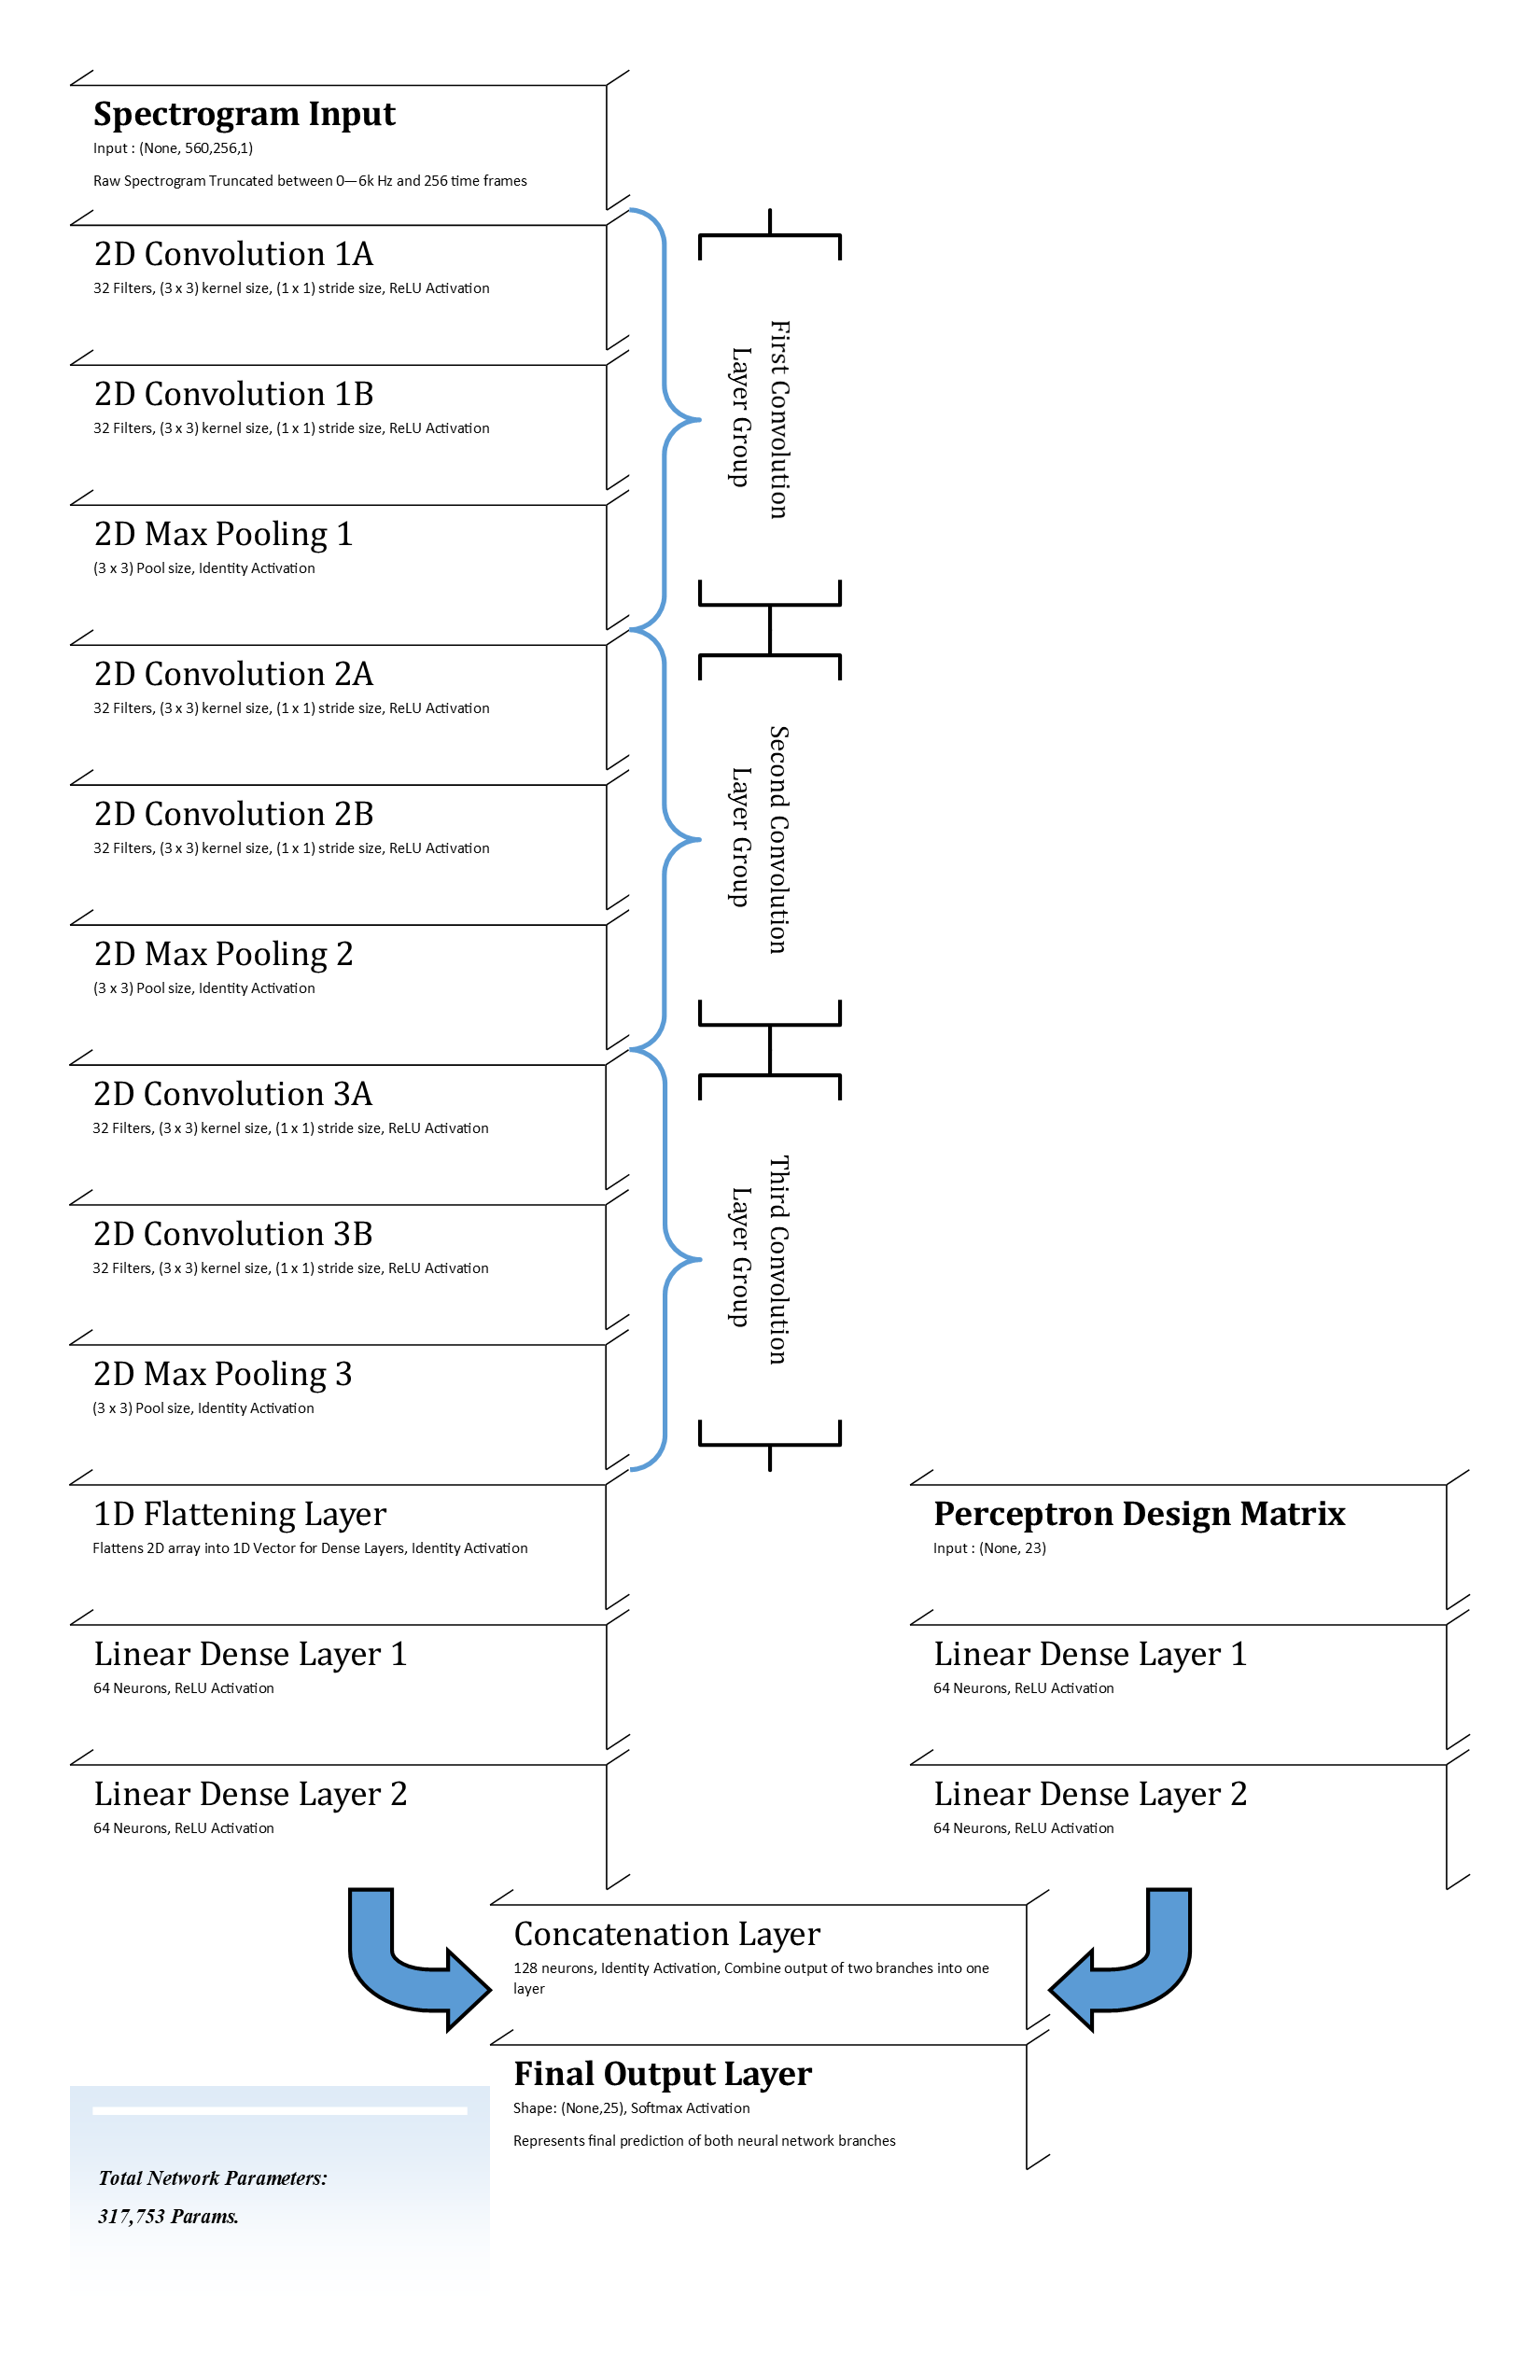
\includegraphics[width=0.45\textwidth]{figures/NeuralNetworkArchitecture.png}
    \caption{Classification architecture for Hybrid Neural Network model}
    \label{fig:Architecture}
\end{figure}

% ================================================================

\subsection{MultiRepresentation Learning}
\label{subsec:Multimodal}

% ================================================================================================================================

\section{Experimental Results}
\label{sec:Results}

% ================================================================================================================================

\section{Discussion and Conclusion}
\label{sec:conclusion}

% ================================================================================================================================

\begin{thebibliography}{9}

\bibitem{Geron}
Geron, Aurelien. \textit{Hands-on Machine Learning with Scikit-Learn and TensorFlow: Concepts, Tools, and Techniques to Build Intelligent Systems}. O'Reilly, 2017.

\bibitem{Goodfellow}
Goodfellow, Ian, et al.\textit{Deep Learning}. MIT Press, 2017.

\bibitem{James}
James, Gareth, et al. An Introduction to Statistical Learning with Applications in R. Springer, 2017

\bibitem{Khan}
Khan, M. Kashif Saeed, and Wasfi G. Al-Khatib. “Machine-Learning Based Classification of Speech and Music.” Multimedia Systems, vol. 12, no. 1, 2006, pp. 55–67., doi:10.1007/s00530-006-0034-0.

\bibitem{Levine}
Levine, Daniel S. Introduction to Neural and Cognitive Modeling. 2nd ed., Routledge, 2000.

\bibitem{Li}
Li, Yingming, and Ming Yang. “A Survey of Multi-View Representation Learning.” Journal of LateX Class Files, vol. 14, no. 8, Aug. 2015. 

\bibitem{Liu}
Liu, Zhu, et al. "Audio Feature Extraction and Analysis for Scene Segmentation and Classification." Journal of VLSI Signal Processing, vol. 20, 1998, pp. 61–79.

\bibitem{McCulloch}
McCulloch, Warren S., and Walter Pitts. "A Logical Calculus of the Ideas Immanent in Nervous Activity." \textit{The Bulletin of Mathematical Biophysics}, vol. 5, no. 4, 1943, pp. 115–133.

\bibitem{Mierswa}
Mierswa, Ingo, and Katharina Morik. ”Automatic Feature Extraction for Classifying Audio Data.” Machine Learning, vol. 58, no. 2-3, 2005, pp. 127–149., doi:10.1007/s10994-005-5824-7.


\bibitem{Ngiam}
Ngiam, Jiquan, et al. "Multimodal Deep Learning." 2011. 

\bibitem{Philharmonia}
Philharmonia Symphony Orchestra home page- \textit{https://philharmonia.co.uk/}

\bibitem{Sahidullah}
Sahidullah, Goutam S. “Design, Analysis and Experimental Evaluation of Block Based Transformation in MFCC Computation for Speaker Recognition.” 18 Nov. 2011.

\bibitem{Tensorflow}
TensorFlow: Large-scale machine learning on heterogeneous systems,
2015. Software available from tensorflow.org.

\bibitem{Virtanen}
Virtanen, Tuomas, et al. \textit{Computational Analysis of Sound Scenes and Events.} Springer, 2018.

\bibitem{UnivIowa}
University of Iowa Electronic Music Studios home page- \textit{http://theremin.music.uiowa.edu/}

\bibitem{Zhang}
Zhang, Tong, and C.-C. Jay Kuo. “Content-Based Classification and Retrieval of Audio.” \textit{Advanced Signal Processing Algorithms, Architectures, and Implementations VIII}, 2 Oct. 1998, pp. 432–443., doi:10.1117/12.325703.

\end{thebibliography}

% ================================================================================================================================

\end{document}